%%%%%%
\chapter{Funções Definidas por Integrais}
%%%%%%%%%%%%%

 A definição de funções por integrais é análoga, sob muitos aspectos, a suas definições
por séries, e nesta seção consideraremos os problemas de derivação
e integração de tais funções.

Seja a função $f(x,\; t)$ definida e contínua no retângulo $\Om
\colon a < s < b,\quad c < t < d$. Então, a integral
$\dst{\int_c^d f(s,\; t)\, dt}$ existe para $a \leq s \leq b$ e define
uma função $F(s)$.

\begin{theoc}{}{1119-34} Dentro das condições enunciadas acima, a
função
 \begin{equation*}
    F(s) =\int_c^d f(s,\; t)\,dt
 \end{equation*}
é contínua em $a < s < b$ ou em símbolo \(F\in C(]a,\; b[)\)
\end{theoc}

\prova Temos
\begin{align*}
|F(s+h)-F(s)|&=\left|\int_c^d[ f(s+h,\; t)-f(s,\; t)]dt \right| \\[2ex]
   & \leq \int_c^d |f(s+h,\; t)-f(s,\;t)|\,dt
\end{align*}

Como $f(s,\; t)$ é \textit{uniformente} contínua no retângulo, ver
Teorema~\ref{thm:1115-14}, podemos, para qualquer $\varepsilon>0$,
exibir um $\de>0$, tal que
\begin{equation*}
  |f(s+h,\; t)-f(s,\; t)|\leq \frac{\varepsilon}{d-c}\quad \text{ quando }
  \quad |h|<\de
\end{equation*}
e com $s$ e $s+h$ no retângulo $R$. Então, $|h|<\de$ implica que
\begin{equation*}
  |F(s+h)-F(s)|\leq \int_c^d\frac{\varepsilon}{d-c}=\varepsilon
\end{equation*}
com isto temos o resultado desejado.\hfill $\square$

Perguntamos, a seguir, se $F(s)$ é diferenciável e se vale a
fórmula natural
\begin{equation*}
 F'(s)=\int_c^d \frac{\partial}{\partial s}f(s,\; t)\, dt
\end{equation*}

Com pequenas restrições, isto resulta verdadeiro.

\begin{theoc}{}{1119-35}
Se $f(s,\; t)$ for contínua em $R$ e se $\dst{\frac{\partial f
}{\partial s}}$ existir e for contínua em $R$, então
\begin{equation*}
F'(s) =\frac{d}{ds}\int_c^d f(s,\; t) dt=\int_c^d \frac{\partial}{\partial s}f(s,\; t)\, dt.
\end{equation*}
\end{theoc}

\prova Calculemos
\begin{equation*}
  \frac{1}{h}[F(s+h,\; t)-F(s)]=\int_c^d\frac{1}{h}[f(s+h,\; t)-f(s)]\,dt.
\end{equation*}

Pelo teorema do valor médio
\begin{equation*}
  \frac{1}{h}[f(s+h,\; t)-f(s,\; t)]=\frac{\partial f(s+\te h,\; t)}{\partial s},
\end{equation*}
em que $\te$ é algum número entre $0$ e $1$. Portanto,
\begin{equation*}
F'(s) = \lim_{h\to 0}\dfrac{F(s + h) - F(s)}{h} = 
\lim_{h \to 0}\int_c^d\dfrac{\partial f (s+\te h,\; t)}{\partial s}\,dt,
\end{equation*}
e como $\dst{\frac{\partial f(s,\; t)}{\partial s} }$ foi suposta
contínua, o Teorema~\ref{thm:1119-34} produz o resultado
desejado.\hfill $\square$

A fórmula do Teorema~\ref{thm:1119-35} pode ser estendida de modo a
permitir limites variáveis na integral, como segue.

\begin{theoc}{}{1119-36}
Sejam $f(s,\; t)$ e $\dst{\frac{\partial\, f}{\partial s}} $
contínuas no retângulo $R\colon a \leq s \leq b$, $c \leq t \leq
d$, e sejam $c(s)$ e $d(s)$ funções continuamente diferenciáveis
com imagem no intervalo fechado $c \leq t \leq d$ (veja a
Figura~\ref{fig-1119-8}). Então,
\begin{align*}
  \frac{d\, F(s)}{ds}=\frac{d}{ds}\int_{c(s)}^{d(s)}f(s,\; t)dt&=\int_{c(s)}^{d(s)}
  \frac{\partial\, f(s,\; t)}{\partial s}dt \\[2ex]
   &\quad+f(s,\; d(s))d'(s)-f(s,\; c(s))c'(s)
\end{align*}
\end{theoc}

\begin{figure}[H]
\centering
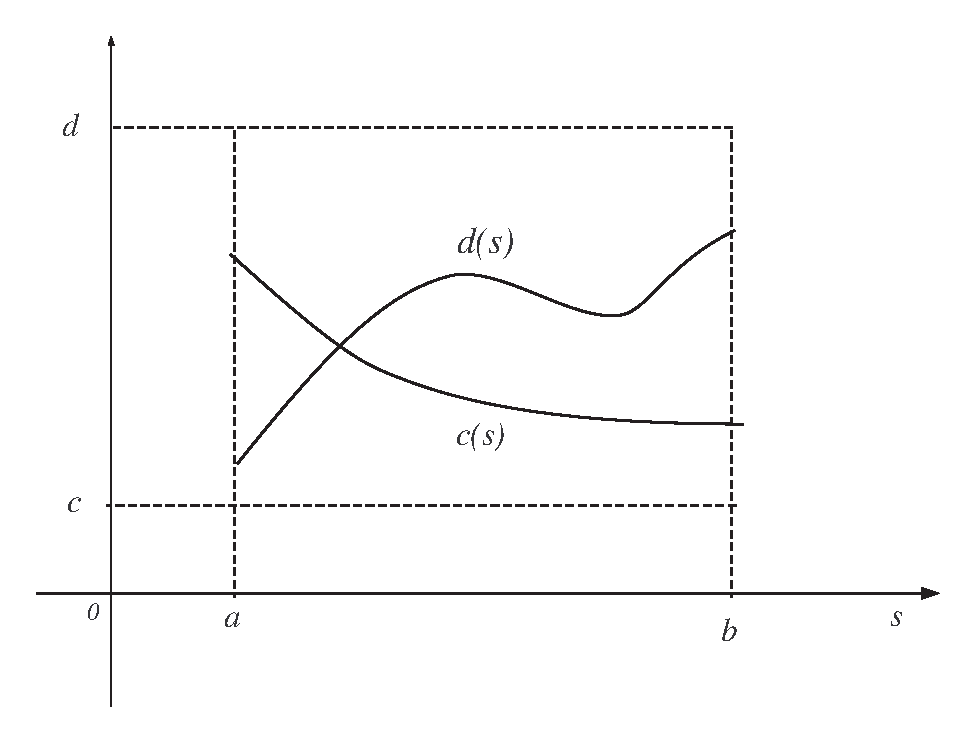
\includegraphics[width=0.65\textwidth]{fig-1119-8.eps}
\caption{Imagem das funções c e d}
\label{fig-1119-8}
\end{figure}

\prova Seja $G (s,\; u,\; v)$ a função definida por
 \begin{equation*}
  G(s,\; u,\;  v)=\int^v_u f(s,\; t)\, dt.
 \end{equation*}

Então, $F(s) = G (s,\; c(s),\; d(s))$, e a regra da cadeia para
funções de várias variáveis fornece,
\begin{align}
 F'(s)=\frac{\partial\, G}{\partial s}(s,\; c(s),\; d(s))&+\frac{\partial\, G}
 {\partial u}(s,\;c(s),\; d(s))\, c'(s)\nonumber  \\[2ex]
   &+\frac{\partial\, G}{\partial v}(s,\;c(s),\; d(s))\, d'(s).\label{1119-21}
\end{align}

Mas, pelo Teorema fundamental do cálculo,
\begin{align*}
  \frac{\partial\, G}{\partial v}(s,c(s),\; d(s)) &= f(s,\; d(s))\\[2ex]
  \frac{\partial\, G}{\partial u}(s,c(s),\; d(s)) &=-f(s,\; c(s))
\end{align*}

e aplicando o Teorema~\ref{thm:1119-35}, obtemos
\begin{equation*}
  \dfrac{\partial\, G}{\partial s}(s,\; c(s),d(s))=\int_{c(s)}^{d(s)}
    \dfrac{\partial\, f(s,\; t)}{\partial s}\, dt
\end{equation*}

Estas equações, juntamente com \eqref{1119-21}, dão a fórmula
desejada, conhecida na literatura como fórmula de Leibnitz.\hfill
$\square$

Voltemos agora nossa atenção para as integrais impróprias; seja
$f$ contínua por partes no intervalo $0\leq x \leq \infty$. Veja também a
seção, espaço das funções contínuas por partes.


\begin{defic}{Convergência}{1119-13} Díz-se que a integral imprópria
$\dst{\int_0^\infty f(x)dx}$ converge, se existe o limite
\begin{equation*}
  \lim_{B\to \infty} \int_0^Bf(x)\, dx
\end{equation*}

Mais precisamente, diz-se que a integral dada converge para $L$, e
escrevemos $\dst{L = \int_0^\infty f(x) dx}$, se para todo $\vep >
0$ existir um número positivo $M$ (dependente, em geral, de
$\vep$), tal que
\begin{equation*}
  \left|L - \int_0^Bf(x)\, dx\right| < \vep\quad  \text{quando}\quad B> M.
\end{equation*}
\end{defic}

De forma semelhante, $\dst{\int_{\mathbb{R}}f(x)\, dx}$ é definida
para funções contínuas por partes em $\mathbb{R}$, pelo limite
duplo
\begin{equation}
\lim_{\substack{A\to\infty\\B\to\infty}}\int_A^B f(x)\, dx
\end{equation}

Agora, se existe $\dst{\int_0^\infty f(s, t) dt}$ para cada valor
de $s$ no intervalo $I$, então ela definirá uma função
\begin{equation*}
  F(s)=\int_0^\infty f(s,\; t)\, dt
\end{equation*}
neste intervalo. A situação aqui, é análoga àquela que se
apresenta ao se definir uma função como o limite (soma) pontual de
uma série infinita; por exemplo, a continuidade de $f(s,\; t)$ na
região $0 \leq t < \infty$, $s$ em $I$, não implica a continuidade
de $F(s)$ em $I$. Por esta razão, estendemos o conceito de
convergência uniforme, como segue.

\begin{defic}{Convergência Uniforme}{1119-14}
A integral $\dst{\int_0^\infty f(s,\; t) dt}$, diz-se convergir
uniformemente para $F(s)$ em $I$ se para todo $\vep > 0$ existir
um número positivo $M$, dependente em geral de $\vep$ mas não de
$s$, tal que
\begin{equation*}
  \left|F(s) - \int^B_0 f(s,\; t) dt\right| < \vep
\end{equation*}
quando $B > M$, e $s$ estiver em $I$.
\end{defic}

Se $\dst{F(s) = \int_0^\infty f(s,\; t)\, dt}$ uniformemente em $I$,
então a integral $\dst{\int_0^B\, f(s,\; t)\, dt}$ poderá ser
compreendida como uma aproximação de $F(s)$ neste intervalo (veja
a discussão correspondente, relativa à convergência uniforme de
séries). Temos, além disso, o

\begin{theoc}{}{1119-37}
Se $f(s,\; t)$ for contínua para $s$ em $I$ e $0 \leq t < \infty$, e
se $\dst{F(s) =\int_0^\infty f(s,\; t)\, dt}$ convergir uniformemente
em $I$, então $F(s)$ será contínua em $I$.
\end{theoc}

\prova Dado $\vep > 0$, escolhamos $B > 0$, tal que
\begin{equation*}
  \left|F(s) - \int^B_A f(s,\; t)\, dt\right| < \vep/3
\end{equation*}
para todo $s$ em $I$. Então,
\begin{align*}
  |F(s+h)-F(s)| & \leq \left|F(s+h) - \int^B_0 f(s+h,\; t)\, dt\right|  \\[2ex]
   &\quad +\left|\int^B_0 f(s+h,\; t)\, dt - \int^B_0 f(s,\; t)\, dt\right| \\[2ex]
   &\quad + \left|\int^B_0 f(s,\; t)\, dt-F(s)\right| \\[2ex]
   &\leq \frac{2\vep}{3}\left|\int_0^B\, f(s+h,\; t)-\int_0^B\, f(s,\; t)\, dt
   \right|.
\end{align*}

Escolhamos agora $\de> 0$ de modo tal que o último termo seja
menor que $\vep/3$ quando $|h| < \de$. (O Teorema~\ref{thm:1119-34}
fornece tal $\de$).\hfill $\square$

O problema de integrar uma função da forma
\begin{equation*}
  F(s)= \int_0^\infty f(s, t)dt, \quad s\quad \text{ em }\quad I,
\end{equation*}
obriga-nos a considerar a questão da permutação da ordem de
integração em integrais iteradas. Recordemos que, para o retângulo
finito $R\colon a \leq s \leq b,\quad c \leq t \leq d$, temos
sempre
\begin{equation*}
  \int_a^b\int_c^d  f(s, t) dt ds =   \int_c^d \int_a^bf(s, t)\, dsdt
\end{equation*}
(contanto que $f$ seja contínua, é claro). Entretanto, este
resultado, em geral, é falso quando as integrações são efetuadas
em intervalos ilimitados.

Para examinar mais de perto esta situação, devemos definir o que
se entende por integrais duplas impróprias e explicar sua relação
com as integrais impróprias iteradas.

\begin{defic}{Convergência de Integral Dupla}{1119-15}
Seja $R$ o primeiro quadrante do plano $s\,t$. Dizemos que a
integral dupla imprópria
\begin{equation*}
  \iint_{R}f (s,\; t)\, dsdt
\end{equation*}
converge para $L$, se para todo $\vep > 0$ existir um número
positivo $M$, tal que
\begin{equation*}
  \left|L -\int_0^B\int_0^A f(s,\; t)\, dsdt\right| < \vep
\end{equation*}
quando $A$, $B$ forem ambos maiores que $M$.
\end{defic}

(Definições análogas são dadas quando $R$ é um semiplano ou plano
inteiro.)

Portanto, se fizermos
\begin{equation*}
  F(A,\; B)=\int_0^B\int_0^A f(s,\, t)\, dsdt
\end{equation*}
então,
\begin{enumerate}[label=(\alph*),leftmargin=1.5cm,ref=(\alph*)]
\item a integral dupla $\dst{\iint_{R}f(s, t)\,dsdt}$ será o limite duplo
\begin{equation*}
  \lim_{\substack{A\to\infty\\B\to \infty}} F(A,\; B);
\end{equation*}
\item  as integrais iteradas serão dadas pelos
limites iterados
\begin{align*}
  \int_0^\infty\int_0^\infty f(s,\; t)\, dsdt &=\lim_{\substack{A\to\infty\\B\to \infty}}  F(A,\; B)\\[2ex]
  \int_0^\infty\int_0^\infty f(s,\; t)\, dtds&=\lim_{\substack{A\to\infty\\B\to \infty}}  F(A,\; B)
\end{align*}
\end{enumerate}

A questão da igualdade das três integrais, então, é justamente um
caso particular do problema correspondente para limites. Portanto,
o seguinte resultado é de interesse neste contexto.

\begin{theoc}{}{1119-38}
Suponhamos exista o duplo limite $\dst{L =
\lim_{\substack{A\to\infty\\ B\to\infty}}F(A,\; B)}$, isto é,
suponhamos que, para todo $\vep > 0$, exista um $M>0$, tal que
$|L-F(A,\; B)| <\vep$ quando $A\geq M$ e $B\geq M$.
\begin{enumerate}[label=(\arabic*)]
\item Se existir $\dst{\lim_{A\to\infty}F(A,\;  B)= L(B)}$ para todo $B$, então
\begin{equation*}
  \lim_{B\to\infty} L(B)= L.
\end{equation*}
\item  Se existir $\dst{\lim_{B\to\infty}F(A,\; B)= L(A)}$ para todo $A$, então
\begin{equation*}
  \lim_{A\to\infty} L(A)= L.
\end{equation*}
\end{enumerate}
\end{theoc}

\prova Basta provar o primeiro item. Ora,
\begin{equation}\label{1119-22}
|L - L(B)| \leq |L - F(A,\; B)| + |F(A,\; B) - L(B)|.
\end{equation}

Assim, dado $\vep >0$, escolhemos $M_1$ de modo tal que $|L - F(A,\; B)| < \vep/2$, quando 
$A \geq M_1$ e $B \geq M_1$. Mantendo $B > M_1$ fixo, podemos encontrar um $M\geq M_1$, tal que 
$|F(A,\; B) - L(B)| < \vep/2$ quando $B\geq M$. Logo, $|L - L(B)| < \vep$, e
como tal pode ser efetuado para qualquer $B \geq M_1$ a
demonstração está encerrada.\hfill $\square$


Reformulado em termos de integrais, o Teorema~\ref{thm:1119-38} afirma
que, se existe  $\dst{L =\iint_{R}f(s,\; t)\, dsdt}$,
então a existência de $\dst{\int_0^\infty f(s,t) dt}$ para todo
$s$ implica que a integral iterada
$\dst{\int_0^\infty\int_0^\infty f(s,\; t)\, dtds}$ existe e é igual a
$L$ (e analogamente ocorre isto com a outra ordem de integração).
Mais interessante, porém, é o problema, inverso, de inferir a
existência da integral dupla a partir da existência, de uma das
integrais iteradas. Para isto, entra mais uma vez a noção de
convergência uniforme e reformulamos a Definição~\ref{def:1119-14} de
maneira apropriada para limites.

\begin{defic}{Convergência Uniforme}{1119-16}
Se $F(A,\; B)$ converge uniformemente para
$L(B)$ quando $A$ vai ao infinito, se para todo $\varepsilon > 0$
existir um número $M> 0$ (dependente, em geral, de $\varepsilon$
mas não de $B$), tal que
\begin{equation*}
  |F(A,\;B)-L(B)| < \varepsilon,\quad \text{ quando }\quad A\geq M
\end{equation*}
\end{defic}

Podemos agora enunciar a principal consequência.

\begin{theoc}{}{1119-39}
Suponhamos que $F (A,\; B)$ convirja uniformemente para $L(B)$
quando $A$ vai ao infinito e que exista $\dst{L =
\lim_{B\to\infty}L(B)}$. Então,
\begin{enumerate}[label=(\arabic*)]
\item $\dst{\lim_{\substack{A\to\infty\\B\to\infty}}F(A,\; B) = L}$, e
\item se existe $\dst{\lim_{B\to\infty}F(A,\; B)=L(A)}$ para todo $A$, então
$\dst{ \lim_{A\to\infty}L(A)=L}$
\end{enumerate}
\end{theoc}

\prova Provaremos o primeiro item. Temos
\begin{equation*}
  |L - F(A,\; B)|\leq |L - L(B)| + |L(B) - F(A,\; B)|.
\end{equation*}

Dado $\varepsilon> 0$, escolhamos $M_1$ de modo que o primeiro
termo do segundo membro seja menor que $\varepsilon/2$ quando $B >
M_1$, e escolhamos $M_2$ (Utilizando-nos da convergência
uniforme), de modo que o segundo termo seja menor que
$\varepsilon/2$ quando $A\geq M_2$. Com $M =\max\{M_1,\; M_2\}$,
teremos $|L - F(A,\; B)| < \varepsilon$, quando $A$, $B$ forem ambos
maiores que $M$.

O segundo item  decorre agora do Teorema~\ref{thm:1119-38}.\hfill
$\square$

Para o caso particular das integrais iteradas impróprias, o teorema acima assume a seguinte forma.
\begin{theoc}{}{1119-40}
Se a integral $\dst{\int_0^\infty f(s,\; t) dt}$ convergir
uniformemente, e se existir a integral iterada
\begin{equation*}
  L = \int_0^\infty\int_0^\infty f (s,\; t) \,dtds
\end{equation*}
então a integral dupla existirá também e satisfará
\begin{equation*}
  \iint_{R}f(s,\; t)\,dsdt=\int_0^\infty\int_0^\infty f(s,\; t)\,dtds.
\end{equation*}

Se, além disso, existir também a integral $\dst{\int_0^\infty f(s,\; t)\, ds}$, então teremos
\begin{equation*}
  \int_0^\infty \int_0^\infty f(s,\; t)\, dtds=\int_0^\infty\int_0^\infty f(s,\; t)\,dsdt
\end{equation*}
\end{theoc}

\begin{coro} Se $f(s,\; t)$ for contínua em $a \leq s \leq b$, $0 \leq t <\infty$, e se
\begin{equation*}
  F(s)=\int_0^\infty f(s, t) dt, \quad a \leq  s \leq  b,
\end{equation*}
sendo a convergência para $F(s)$ uniforme em $ a \leq s \leq b$, então
\begin{equation*}
\int_a^b F(s)\, ds = \int_a^b\int_0^\infty f(s,\; t)\,dtds
=\int_0^\infty \int_a^b f(s,\; t)\, dsdt.
\end{equation*}
\end{coro}

\prova Precisaremos apenas aplicar o teorema à função
$\hat{f}(s,\; t)$, definida em $0 \leq s < \infty$, $0 \leq t<\infty$
por
\begin{equation*}
 \hat{f}(s,\; t)=
  \begin{cases}
    f(s,\; t) & \text{ se},\quad a\leq s\leq b \\[2ex]
    0 & \text{ para outros valores de} \quad s
  \end{cases}
\end{equation*}

Porque, então, $\dst{\int_0^\infty\hat{f}(s,\; t)\, dt}$  convergirá
uniformemente em $0 \leq s <\infty$  para a função
\begin{equation*}
 \hat{F}(s)=
  \begin{cases}
    F(s) & \text{ se},\quad a\leq s\leq b \\[2ex]
    0 & \text{ para outros valores de} \quad s
  \end{cases}
\end{equation*}
e
\begin{equation*}
  \int_0^\infty\hat{f}(s,\; t)ds=\int_a^b\hat{f}(s,\; t)ds=\int_a^b f(s,\; t)\, ds
\end{equation*}
existirá.\hfill $\square$

Os teoremas apresentados acima tratam do problema de integrar
funções definidas por integrais impróprias. Uma consequência útil,
concernente à derivação de tais funções, é a seguinte,
\begin{theoc}{}{1119-41}
Se $\dst{\frac{\partial f(s,\; t)}{\partial s}}$ for contínua por
partes em, $a \leq s \le b$ para cada $t$, e se
\begin{equation*}
F(s)=\int_0^\infty\,f(s,\; t)\,dt \quad \text{ e }\quad
\int_0^\infty \frac{\partial f(s,\; t)}{\partial s}\, dt
\end{equation*}
convergirem uniformemente em $a \leq s \leq b$, então
\begin{equation*}
  F'(s)=\int_0^\infty \frac{\partial f(s,\; t)}{\partial s}\, dt
\end{equation*}
\end{theoc}

\prova Seja
$\dst{H(s)=\int_0^\infty\frac{\partial f(s,\; t)}{\partial s}\, dt }$.
Então,
\begin{align*}
  \int_a^u\,H(s)ds &=\int_a^u\int_0^\infty \frac{\partial\,f(s,\; t)}{\partial s}\, dtds
  = \int_0^\infty\int_a^u \frac{\partial\,f(s,t)}{\partial s}\, dsdt   \\[2ex]
  & =\int_0^\infty [f(u,\; t) - f(a,\; t)] dt  \\[2ex]
   &=F(u) - F(a),
\end{align*}
donde $H(u) = F'(u)$ por derivação.\hfill $\square$

%%%%%
\section{Aplicações}
%%%%%

Um dos principais exemplos no texto de uma função definida por uma
integral é a transformada de, Laplace
\begin{equation}\label{1119-23}
\mathcal{L}[f](s)= \int_0^\infty e^{-st}f(t)\,dt = F(s)
\end{equation}
de uma função contínua por partes. Como $f$ não precisa de ser
contínua, a convergência uniforme de \eqref{1119-23} (estabelecida
abaixo) não é suficiente para estabelecer a continuidade de
$F(s)$. Contudo, para funções $f$ de ordem exponencial, temos,
para $h > 0$,
\begin{align*}
  |F(s+h)-F(s)| & =\left|\int_0^\infty (e^{-(s+h)t}-e^{-st})f(t)\, dt  \right|\\[2ex]
  &= \left|\int_0^\infty (e^{-ht}-1)e^{-st}f(t)\, dt  \right|\\[2ex]
  &\leq \int_0^\infty (1-e^{-ht})e^{-st}|f(t)|\, dt
\end{align*}

Portanto, se $\al$, $M$ são constantes quaisquer escolhidas de
modo que $|f(t)| \leq  Me^{s_1t}$ segue-se que, para $s > \al$,
\begin{align*}
  |F(s+h)-F(s)| &\leq M \int_0^\infty (1-e^{-ht})e^{-(s-\al)t}dt  \\[2ex]
   &=M\left[\frac{1}{s-h}-\frac{1}{h+s-\al} \right],
\end{align*}
 e, consequentemente, que $F(s + h) - F(s)$ tende para zero, quando
$h$ vai ao zero por valores positivos. Ligeira modificação no
argumento dá o mesmo resultado, se $h$ vai ao zero por valores
negativos, e assim estará comprovada a continuidade de $F(s)$ para
$s> \al$. Demonstramos, assim, o seguinte teorema.

\begin{theoc}{}{1119-42} 
Se $f$ for contínua por partes em $0 \leq t <\infty$
e for de ordem exponencial, e se $\al_o$ for o ínfimo do conjunto
de números reais a para os quais $|f(t)|\leq Me^{s_1t}$ (para
alguma constante $M$), então $\mathcal{L}[f]$ será contínua em
$\al_{0} < s < \infty$
\end{theoc}

\begin{obs} O número $\al_o$, chamado, algumas vezes, de ordem de $f$, é
maior ou igual à abscissa de convergência $s_{0}$ de $f$. No
entanto, como foi mostrado em seu lugar, podemos ter $s_{0}<\al_{0}$.
\end{obs}

Finalmente, justifiquemos a fórmula
\begin{equation*}
  \dfrac{d^n}{ds^n}\mathcal{L}[f](s)=\dfrac{d^n}{ds^n}\int_0^\infty e^{-st}f(t)\, dt
  =(-1)^n\int_0^\infty t^ne^{-st}f(t)\,dt
\end{equation*}
 dada em seção anterior desta obra, mostrando que cada uma das integrais
\begin{equation}\label{1119-24}
  \int_0^\infty t^ne^{-st}f(t)\, dt,\quad n = 0,\; 1,\; 2,\ldots
\end{equation}

converge uniformemente em $\al \leq  s < \infty$ onde $\al <
\al_o$ (veja Teorema~\ref{thm:1119-42} para a definição de $\al_{0}$).
De fato, escolhendo $s_1$ ($\al_{0} < s_1 < \al$) e $M$, de modo que
$|f(t)|\leq Me^{s_1t}$, temos, para $s> \al$,

\begin{align*}
\left|\int_A^\infty t^n e^{-st}f(t)\, dt \right| &\leq M\int_A^\infty t^n e^{(s-s_1)t}\, dt\\[2ex]
&\leq M\int_A^\infty t^n e^{(\al-s_1)t}\, dt
\end{align*}


Mas a última expressão tende para zero quando $A$ vai ao infinito
($t^n$ é de ordem exponencial), e como ela não depende de $s$,
está demonstrada a convergência uniforme de \eqref{1119-24} em
$\al \leq s < \infty$. Em vista do Teorema~\ref{thm:1119-41}, pode-se
efetuar qualquer quantidade de derivações, de $\mathcal{L}[f](s)$
derivando-se sob o sinal de integral. \hfill $\square$